\documentclass[tikz,border=10pt]{standalone}
\usepackage{tikz}
\usepackage{babel}

\begin{document}

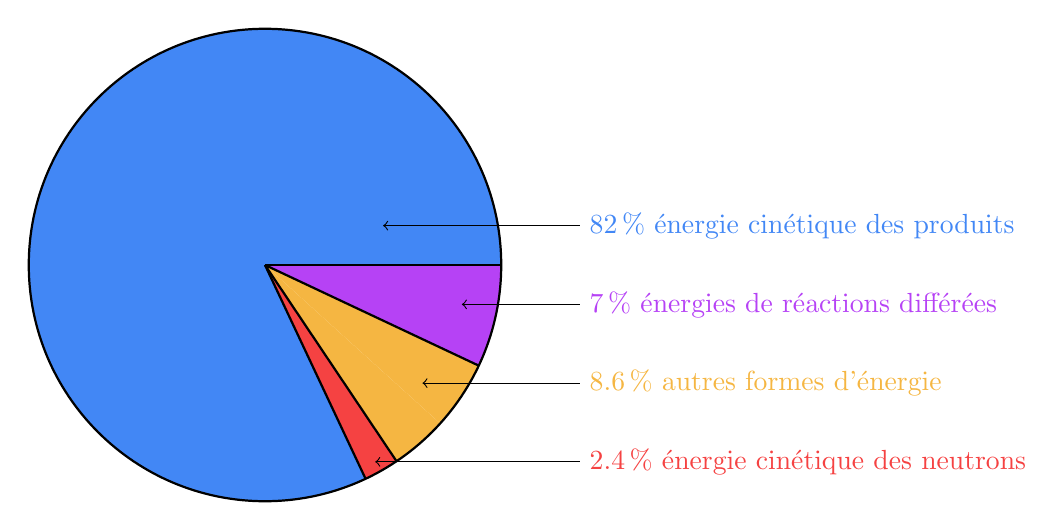
\begin{tikzpicture}


% Définition des données
\def\energyA{82} % Énergie cinétique des fragments de fission
\def\energyB{2.4} % Énergie cinétique des neutrons
\def\energyC{3.9} % Énergie des rayons gamma instantanés
\def\energyD{4.7} % Énergie des neutrinos
\def\energyE{7}   % Énergies différées (radioactivité β et γ)

% Couleurs pour chaque section
\definecolor{colorA}{RGB}{66, 135, 245} % Bleu (fragments)
\definecolor{colorB}{RGB}{245, 66, 66}  % Rouge (neutrons)
\definecolor{colorC}{RGB}{245, 182, 66} % Orange (gamma instantanés)
\definecolor{colorD}{RGB}{245, 182, 66} % Vert clair (neutrinos)
\definecolor{colorE}{RGB}{182, 66, 245} % Violet (énergies différées)

% Positions angulaires cumulatives
\def\aA{\energyA/100*360}
\def\aB{\aA + \energyB/100*360}
\def\aC{\aB + \energyC/100*360}
\def\aD{\aC + \energyD/100*360}


% Diagramme circulaire
\begin{scope}
    % Secteurs
    \fill[colorA] (0,0) -- (0:3) arc[start angle=0, end angle=\aA, radius=3] -- cycle; % Fragments
    \fill[colorB] (0,0) -- (\aA:3) arc[start angle=\aA, end angle=\aB, radius=3] -- cycle; % Neutrons
    \fill[colorC] (0,0) -- (\aB:3) arc[start angle=\aB, end angle=\aC, radius=3] -- cycle; % Gamma instantanés
    \fill[colorD] (0,0) -- (\aC:3) arc[start angle=\aC, end angle=\aD, radius=3] -- cycle; % Neutrinos
    \fill[colorE] (0,0) -- (\aD:3) arc[start angle=\aD, end angle=360, radius=3] -- cycle; % Énergies différées

    % Rayons pour séparer les régions
    \draw[thick] (0,0) -- (0:3);
    \draw[thick] (0,0) -- (\aA:3);
    \draw[thick] (0,0) -- (\aB:3);
    \draw[thick] (0,0) -- (\aD:3);
    % Légendes avec flèches
    \draw[<-] (1.5,0.5) -- (4,0.5) node[right,colorA]
    {82\,\% énergie cinétique des produits};
    \draw[<-] (1.4,-2.5) -- (4,-2.5) node[right,colorB]
    {2.4\,\% énergie cinétique des neutrons};
    \draw[<-] (2,-1.5) -- (4,-1.5) node[right,colorC]
    {8.6\,\% autres formes d'énergie};
    \draw[<-] (2.5,-.5) -- (4,-0.5) node[right,colorE] {7\,\%
      énergies de réactions différées};

    % Cercle extérieur pour l'esthétique
    \draw[thick] (0,0) circle(3);



\end{scope}


\end{tikzpicture}

\end{document}
